\chapter{观测、暗物质与宇宙学拟合}

\lectureoverview{观测只有与宇宙学模型联系起来之后才获得意义。我们从弗里德曼方程和三种均匀空间几何出发，把当今的宇宙预算整理为辐射、物质、真空能量和曲率，并重构出为什么开放宇宙一度显得不可避免。接着，星系旋转曲线揭示出缺失的引力物质，并引向冷的、弱相互作用晕的动力学。最后，红移、亮度和源计数把试探性的膨胀历史变成可观测的曲线。旧的物质加曲率模型失败了；物质分数接近\(0.3\)、真空分数接近\(0.7\)以及非常小的曲率，给出了本讲的成功拟合。}

\section{把观测放回方程中}

天文事实不能孤立地解释。我们首先需要那些告诉我们哪些观测组合能区分一个宇宙与另一个宇宙的方程。对于均匀且各向同性的宇宙，起点是弗里德曼方程，
\begin{equation}
\left(\frac{\dot a}{a}\right)^2
=
\frac{8\pi G}{3}\rho-\frac{k}{a^2}.
\label{eq:c06-friedmann}
\end{equation}
量
\begin{equation}
H(t)=\frac{\dot a(t)}{a(t)}
\label{eq:c06-hubble}
\end{equation}
是哈勃\emph{函数}。它的当前值\(H_0\)习惯上被称为哈勃常数，但\(H(t)\)在宇宙历史中并非常数。当天文学家给出以千米每秒每百万秒差距为单位的值时，他们给出的就是\(H_0\)。

归一化曲率标签只取三个值，
\begin{equation}
k\in\{+1,0,-1\},
\end{equation}
分别对应球面、平坦和双曲空间几何。常见的FRW度规可以写成
\begin{equation}
ds^2=-dt^2+a(t)^2\left[dr^2+\xi(r)^2d\Omega_2^2\right],
\label{eq:c06-frw}
\end{equation}
其中
\begin{equation}
\xi(r)=
\begin{cases}
\sin r, & k=+1,\\
r, & k=0,\\
\sinh r, & k=-1.
\end{cases}
\label{eq:c06-xi}
\end{equation}
这种记号将承担两项任务。它把三种几何打包进一个度规，并且稍后给出球的面积，从而给出径向壳层中的源数目。因此，选择\(k\)以及关于\(a(t)\)的方程，已经是一个具有观测后果的模型。

\section{当今的宇宙预算}

在所讨论的模型中，能量密度有三个主要组成部分：辐射、非相对论物质和真空能量。把曲率列入同一本账，得到
\begin{equation}
\frac{C_r}{a^4}
+\frac{C_m}{a^3}
+\Lambda
-\frac{k}{a^2}
=H^2.
\label{eq:c06-budget}
\end{equation}
这里\(\Lambda\)采用了上一讲的归一化，\(\Lambda=(8\pi G/3)\rho_{\rm vac}\)。辐射按\(a^{-4}\)稀释，物质按\(a^{-3}\)稀释，真空能量不稀释，而曲率按\(a^{-2}\)缩放。曲率不是一种物质能量密度，但把它与其他项并列，使当今的约束变得透明：四项贡献之和必须等于\(H_0^2\)。

用下式定义它们当今的分数
\begin{equation}
\begin{aligned}
\Omega_r&=\frac{C_r/a_0^4}{H_0^2},
&\qquad
\Omega_m&=\frac{C_m/a_0^3}{H_0^2},\\
\Omega_\Lambda&=\frac{\Lambda}{H_0^2},
&
\Omega_k&=\frac{-k/a_0^2}{H_0^2}.
\end{aligned}
\label{eq:c06-omegas}
\end{equation}
于是
\begin{equation}
\boxed{\Omega_r+\Omega_m+\Omega_\Lambda+\Omega_k=1.}
\label{eq:c06-sum-rule}
\end{equation}
这些\(\Omega\)是今天取值的比率，而不是与时间无关的常数。还要注意符号约定：\(k=-1\)给出正的\(\Omega_k\)。

\subsection{最初几项如何测量}

哈勃通过比较退行红移与距离，得到了局部膨胀率。红移在低\(z\)下给出速度；经过校准的亮度给出距离。他最初的数值大错特错，但方法是对的。由于那些星系相对较近，这一测量并未探测宇宙历史的很大一部分，因而可以把\(H\)当作其当前值。

\begin{classroomqa}
\audiencequestion{除非内禀亮度已经知道，亮度如何能确定距离？}
\lecturerresponse{它不能一步做到。宇宙距离阶梯从近邻恒星的视差开始。在该校准区域内的造父变星揭示出周光关系，并成为更远距离的标准烛光。相互重叠的校准把阶梯向外延伸，而超新星为后来使用的宇宙学红移提供了最好的烛光。因此，距离是由一连串标准推断出来的，而不是任意假设每个天体都同样发光。 \lecturetimestamp{00:10:00--00:11:32}}
\end{classroomqa}

\begin{classroomqa}
\audiencequestion{尽管\(C_r\)和\(C_m\)的密度会变化，它们仍是常数吗？}
\lecturerresponse{是的。系数保持固定，而因子\(a^{-4}\)和\(a^{-3}\)承载时间依赖。真空能量是常数，曲率按\(a^{-2}\)缩放。正是这些不相等的幂，使得分数贡献从一个时代到另一个时代发生变化。 \lecturetimestamp{00:11:35--00:12:02}}
\end{classroomqa}

辐射项可以在局部由光子背景测量。其中大部分是宇宙微波背景，其当今能量密度与其他重要组成部分相比微不足道。需要足够大的平均体积，但无需沿过去光锥作长途回溯，就能确定\(\Omega_r\)在今天可以忽略。

可见物质是根据星系、恒星族、氢以及星际气体估算出来的。这些方法属于技术性的，而非概念上晦涩难懂：确定典型的恒星和气体含量，将其对星系求和，再在一个大体积上取平均。讲座引用了旧的粗略尺度，即每立方米一个质子质量。这比辐射密度大得多，但仍然稀薄得惊人。

\begin{classroomqa}
\audiencequestion{在这种核算中，暗物质又如何呢？}
\lecturerresponse{它即将出现，但首先我们有意重建仅基于发光物质的旧推断。历史顺序很重要：它恰好显示出暗物质纠正了哪个表面结论，以及它没有填补哪个缺口。\lecturetimestamp{00:15:08--00:15:40}}
\end{classroomqa}

\section{为什么开放宇宙曾一度显得必要}

在旧的图景中，辐射被正确地判定为可忽略，真空能量被设为零，而物质仅指通过电磁辐射可见的物质。由此得到的估计大致为
\begin{equation}
\Omega_r\simeq0,
\qquad
\Omega_\Lambda=0,
\qquad
\Omega_m^{\rm luminous}\sim\frac{1}{20}\text{--}\frac{1}{30}.
\end{equation}
于是求和规则似乎迫使
\begin{equation}
\Omega_k\simeq1.
\end{equation}
由于正的曲率贡献意味着\(-k/a_0^2>0\)，这就暗示了\(k=-1\)：一个开放的、负曲率的宇宙。这些数字是对旧论证的重建，而非现代的参数估计。

为了解释曲率尺度，回到物质主导的解
\begin{equation}
a(t)\propto t^{2/3}.
\end{equation}
求导并除以\(a\)，得到
\begin{equation}
H(t)=\frac{\dot a}{a}=\frac{2}{3t}.
\label{eq:c06-matter-h}
\end{equation}
在当前年龄\(T\)时，
\begin{equation}
H_0\simeq\frac{2}{3T}.
\end{equation}
因此哈勃时间与宇宙年龄同量级。辐射主导的对比，
\begin{equation}
a(t)\propto t^{1/2},
\qquad
H(t)=\frac{1}{2t},
\end{equation}
表明这种年龄倒数关系并非尘埃所特有。

\begin{figure}[htbp]
\centering
\includegraphics[width=0.72\textwidth]{lecture_06_figure_02.png}
\caption{物质时代的板书回顾。可见的书写内容包含\(a\sim t^{2/3}\)和\(\dot a/a=2/(3t)\)；讲师遮住了黑板上剩余的部分，因此不将任何隐藏方程归因于该画面。}
\label{fig:c06-age-board}
\lectureframe{00:24:41.615}
\end{figure}

\begin{classroomqa}
\audiencequestion{哈勃常数具有什么单位，光速又在哪里？}
\lecturerresponse{由于\(H\)将速度与距离联系起来，它具有时间的倒数单位。它可以用每秒的倒数、每年的倒数，或天文学家所用的等价单位千米每秒每百万秒差距来引用。关系式\(H\sim1/T\)不需要额外的\(c\)。只有当时间\(c\)被转换为诸如\(T\)这样的长度时，才会出现一个\(cT\)因子。\lecturetimestamp{00:22:50--00:24:25}}
\end{classroomqa}

哈勃最初的值\(H_0\)大约大了一个数量级，因此相应的哈勃年龄太短，在讲座四舍五入的比较中约为十亿年而非一百亿年。更好的校准修正了这个数字，却没有改变\(H_0^{-1}\)是一个宇宙时间尺度这一逻辑。

旧的曲率推断现在读作
\begin{equation}
\frac{1}{a_0^2}\sim H_0^2\sim\frac{1}{T^2}.
\end{equation}
在单位\(c=1\)下，曲率半径\(a_0\)因此被认为与年龄\(T\)同量级；恢复普通单位后，它与\(cT\)同量级。讲座立即撤回这一点，不将其作为关于真实宇宙的陈述。这是几十年前在舍弃当时被认为可忽略的项之后所得到的结论。

\begin{classroomqa}
\audiencequestion{如果曲率本应在今天占主导，为什么要使用物质主导定律\(a\propto t^{2/3}\)？}
\lecturerresponse{因为物质按\(a^{-3}\)缩放，而曲率仅按\(a^{-2}\)缩放。在较小的\(a\)下，物质占优。曲率只能在晚期变得重要，因此物质主导仍然描述了已流逝历史的大部分，并使\(H_0\)保持在\(1/T\)的量级。完整的混合解会修正数值因子，而不会抹去时间尺度论证。\lecturetimestamp{00:49:20--00:50:17}}
\end{classroomqa}

\section{来自星系动力学的暗物质}

有两种可操作的方法来清点物质。一种是清点发出或吸收光的物质。另一种是从引力推断质量。奥尔特在1930年代初发现了异常的星系动力学，兹威基在星系团中发现了类似的质量差异。证据表明，引力物质超过了发光物质。普通带电物质会辐射并碰撞；缺失的成分首先是通过其引力作用而被认识的。

\begin{classroomqa}
\audiencequestion{发光物质是否包括弥散气体和中心黑洞？}
\lecturerresponse{弥散气体在其数量能够从其电磁行为推断出来的范围内被包括在内。中心超大质量黑洞可能被包括在已知质量预算中，但它只占星系总质量的一小部分，并且集中在中心。它无法解释一个在发光中心之外很远仍持续存在的差异。\lecturetimestamp{00:29:50--00:31:14}}
\end{classroomqa}

考虑一颗大致沿半径为\(r\)的圆轨道运动的恒星。如果几乎全部质量\(M\)都集中在星系中心附近，牛顿定律将给出
\begin{equation}
\frac{GM}{r^2}=\frac{v^2}{r},
\end{equation}
因而
\begin{equation}
v^2=\frac{GM}{r},
\qquad
v(r)\propto r^{-1/2}.
\label{eq:c06-kepler}
\end{equation}
这就是在中心质量分布之外所预期的开普勒衰减。

\begin{figure}[htbp]
\centering
\includegraphics[width=0.78\textwidth]{lecture_06_figure_03.png}
\caption{从中心质量过渡到包含质量\(M(r)\)时的转动曲线板书。只有\(MG\)、分数线、轨道草图以及曲线草图的部分可见；方程~\eqref{eq:c06-kepler}来自口头推导。}
\label{fig:c06-rotation-board}
\lectureframe{00:34:53.642}
\end{figure}

\begin{figure}[htbp]
\centering
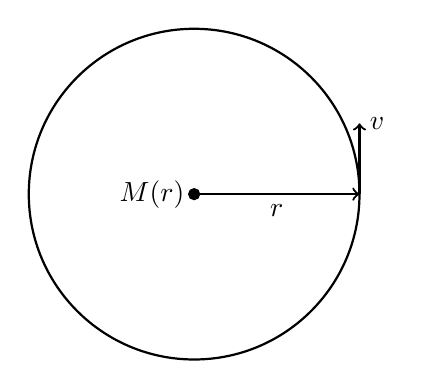
\begin{tikzpicture}[scale=1.0]
\filldraw (0,0) circle (2pt) node[left] {\(M(r)\)};
\draw[thick] (0,0) circle (2.1);
\draw[->,thick] (0,0)--(2.1,0) node[midway,below] {\(r\)};
\draw[->,thick] (2.1,0)--(2.1,0.9) node[right] {\(v\)};
\end{tikzpicture}
\caption{用于从测得的转动速率推断包含质量的圆轨道构造。}
\label{fig:c06-orbit-redraw}
\end{figure}

观测到的星系转动曲线并不以这种方式下降；在相当大的径向范围内它们近似平坦。将固定的中心质量替换为包含质量\(M(r)\)：
\begin{equation}
\frac{G M(r)}{r^2}=\frac{v(r)^2}{r}.
\end{equation}
如果\(v(r)\)近似恒定，那么
\begin{equation}
\boxed{M(r)\propto r.}
\label{eq:c06-enclosed-mass}
\end{equation}
这里指的是半径\(r\)以内的总质量，而不是局部密度。引力质量继续增长，远远超出大部分星光集中的区域。垂直于星系盘的运动进一步表明存在近似球形的分布：一个暗晕，而不是第二个薄盘。

\begin{classroomqa}
\audiencequestion{是否存在一个简单的理论来解释为什么转动曲线如此平坦？}
\lecturerresponse{在这一论证中没有。星系形成的模拟或许会使这样的轮廓变得自然，但讲座并未声称有一个简短的推导。可靠的陈述是观测性的：近似恒定的\(v\)意味着包含质量近似线性增长。不应把这一关系的简洁误认为对星系形成的初等解释。\lecturetimestamp{00:35:58--00:37:33}}
\end{classroomqa}

\begin{classroomqa}
\audiencequestion{旋臂是否只是由变化的角速度\(v/r\)产生的物质风车？}
\lecturerresponse{没有简单的风车图像可行。可见的图案不必与单个恒星一起旋转；密度波或恒星形成波的描述是可能的解释之一。讲座利用这一不确定性，将稳健的暗晕推断与更复杂的旋臂结构问题区分开来。\lecturetimestamp{00:37:35--00:38:34; 00:47:03--00:47:47}}
\end{classroomqa}

推断出的暗质量是发光质量的数倍，讲座中只将其作为大约五到十之间的数量级因子给出。暗晕还延伸到可见星系之外。这些是刻意粗略的历史尺度，而不是适用于每个系统的精确普适比值。

\section{暗物质必须是什么样的}

为什么普通物质形成明亮致密的盘，而暗物质却留在宽广的晕中？发光物质可以通过电磁碰撞和辐射失去机械能。一旦它耗散能量，引力就能把它拉入更致密的构型。暗物质似乎是电中性的，并且相互作用弱得多。它的粒子在晕中穿行时几乎没有碰撞或辐射，因此即使在数十亿年间也不会失去足够的能量而沉降到发光盘中。星系运动产生的引力辐射太弱，无法提供另一种冷却机制。

\begin{classroomqa}
\audiencequestion{弱相互作用是否意味着暗物质遵循不同的引力定律？}
\lecturerresponse{不。假定它以通常的方式产生引力。这里的弱相互作用指的是非引力碰撞和电磁辐射的缺失或极大抑制。两个暗粒子仍然通过引力相互吸引；这种吸引组织成一个晕，但不能有效地耗散轨道能量。\lecturetimestamp{00:42:36--00:43:35}}
\end{classroomqa}

\begin{classroomqa}
\audiencequestion{哪些观测表明这不仅仅是一个星系转动曲线的特殊性？}
\lecturerresponse{证据出现在多个尺度上：星系内恒星的运动、垂直于星系平面的运动、星系之间的相互作用，以及整个星系团的动力学。奥尔特和兹威基的例子是同一个缺失引力问题的不同表现。\lecturetimestamp{00:42:00--00:42:36}}
\end{classroomqa}

\begin{classroomqa}
\audiencequestion{暗物质是否应该聚集在黑洞和星系中心周围？}
\lecturerresponse{它确实会朝着引力中心变得更致密，但历史顺序很可能与晕围绕预先存在的黑洞形成相反。暗晕形成了巨大的引力势阱；随后重子物质落入其中，形成了星系、恒星和中心黑洞。黑洞只占质量的一小部分。尽管如此，对湮灭产物的搜寻仍朝向星系中心，因为预期那里的暗物质密度更高。\lecturetimestamp{00:43:36--00:45:43}}
\end{classroomqa}

\begin{classroomqa}
\audiencequestion{暗物质是气体、尘埃、致密团块，还是孤立粒子？其中一些会不会被束缚在太阳附近？}
\lecturerresponse{其微观本质尚不清楚，但普通尘埃由电磁力束缚，而暗物质似乎恰恰缺乏这类相互作用。因此，默认的粒子图像是一群稀薄的单个粒子。其中一些可能被引力聚集在太阳附近，但它们的密度远不足以与太阳引力相抗衡，也不会扰动行星动力学。\lecturetimestamp{00:45:43--00:47:02; 00:58:41--00:59:29}}
\end{classroomqa}

第二个核心要求是暗物质必须成团。具有相对论性随机速度的热粒子群会抵抗引力聚集；而冷粒子群则能落入势阱。普通轻中微子会表现为热暗物质，无法提供所需的星系主要成分。在此语境下，\emph{冷}指的是在局部宇宙学参考系中非相对论性，而非字面意义上的实验室零温度。

\begin{classroomqa}
\audiencequestion{冷成团的要求是否限定了暗物质的质量范围？}
\lecturerresponse{这取决于量子统计和产生历史。极轻的费米子不能全部占据同一个慢速态，因而受到强烈限制。极轻的玻色子则可以占据相干的玻色凝聚态；轴子就是本讲给出的例子。另一种可能是，较重的弱相互作用粒子无需凝聚也能是冷的。因此，这一论证并不能给出一个与模型无关的单一质量界限。\lecturetimestamp{00:53:17--00:54:52; 00:56:42--00:58:05}}
\end{classroomqa}

\begin{classroomqa}
\audiencequestion{加速器难道不应该已经发现这些粒子了吗？}
\lecturerresponse{只有在附加假设下才会如此。如果这些粒子具有大致弱相互作用的截面，且质量在加速器可及范围内，那么对撞机产生或许是可能的。本讲对即将获得信息的预期明确是推测性的，并且带有历史时代印记。粒子也可能太重，或者相互作用太微弱，以至于现有实验无法探测。\lecturetimestamp{00:54:52--00:55:54}}
\end{classroomqa}

\begin{classroomqa}
\audiencequestion{暗物质会不会只是存在于一个看不见的额外维度中？}
\lecturerresponse{讨论中并不需要这样的机制。暗物质已经通过引力被观测到，它可能只是由与普通物质几乎不发生相互作用的奇异粒子组成。称一种相互作用为弱，并不等于把这些粒子置于可观测时空之外。\lecturetimestamp{00:55:54--00:56:41}}
\end{classroomqa}

修改引力而不是添加看不见的物质，是一个逻辑上的替代方案。本讲的判断是：当时没有任何同样简单的修改能够在所有相关尺度上解释这些证据，同时保留已经成功的太阳系定律。因此粒子解释更受青睐，但其微观物理仍然未知。

\section{暗物质并不能补上旧的预算}

暗物质把物质贡献放大了数倍，但发光物质与\(H_0^2\)之间的旧差距约为二十五倍。因此它缩小了差距，却并未
\begin{equation}
\frac{C_m}{a_0^3}=H_0^2.
\end{equation}
在旧的、没有\(\Lambda\)的图像中，仍然需要一个正的曲率预算项，因而需要\(k<0\)。这样的开放模型在逻辑上并无不一致之处；关键在于，仅靠暗物质并不能选出那个现代答案。

\begin{classroomqa}
\audiencequestion{在现代拟合之前，宇宙学家实际上如何看待曲率？}
\lecturerresponse{证据令人困惑，而对闭合、有界宇宙的偏好有时会与物质预算相冲突。一旦把旧假设一致地结合起来，负曲率就是自然的推论。那个历史共识仍然是暂时的，因为无论暗物质还是真空能，都尚未以今天的方式被可靠地纳入其中。\lecturetimestamp{00:50:17--00:51:50}}
\end{classroomqa}

因此，我们必须检验候选模型，而不是从一条预算线推断其真伪。一个模型由曲率选择\(k\)和膨胀历史\(a(t)\)组成，等价地说，由一组物质状态方程和当前参数组成，并由它们计算出\(a(t)\)。旧的候选模型是物质加负曲率，辐射可忽略，且没有宇宙学常数。

\section{把几何变成可观测量}

\subsection{冻结几何中的源计数与亮度}

暂时忽略宇宙演化。在均匀宇宙中，共动壳层内的源数目正比于其面积：
\begin{equation}
dN\propto \xi(r)^2\,dr.
\label{eq:c06-shell-count}
\end{equation}
因此
\begin{equation}
dN\propto
\begin{cases}
\sin^2r\,dr, & k=+1,\\
r^2\,dr, & k=0,\\
\sinh^2r\,dr, & k=-1.
\end{cases}
\end{equation}
在大的\(r\)下，负曲率情形按\(\sinh^2r\sim e^{2r}\)增长，远快于平坦情形的\(r^2\)律。因此，负曲率预言源数目随距离异常迅速地增加。

同一面积决定了接收到的通量。在平坦静态空间中，标准源给出
\begin{equation}
F\propto\frac{1}{r^2}.
\end{equation}
在双曲空间中，辐射扩散所经过的球面增长得更快，因此通量下降得更快。讲座有时把这一观测量称为光度；这里\(F\)表示亮度或通量，而内禀光度属于源本身。因此，计数与亮度结合起来可以区分空间几何。

\subsection{红移与过去光锥}

真实宇宙在演化，向外看就意味着向过去看。在\(t_{\rm em}\)发出的光在尺度因子从\(a(t_{\rm em})\)增长到\(a_0\)的过程中被拉伸：
\begin{equation}
1+z
=\frac{\lambda_{\rm obs}}{\lambda_{\rm em}}
=\frac{a_0}{a(t_{\rm em})}.
\label{eq:c06-redshift}
\end{equation}
等价地，
\begin{equation}
z=\frac{\lambda_{\rm obs}}{\lambda_{\rm em}}-1.
\end{equation}
我们过去光锥上的不同点同时对应不同的共动半径和不同的发射时刻。膨胀改变波长；多普勒频移和引力频移是其他物理机制，但宇宙学膨胀才是这里所讨论的效应。

\begin{classroomqa}
\audiencequestion{为什么\(z\)的定义中包含减一？}
\lecturerresponse{这是一个历史约定，选择它是为了使未发生红移的源具有\(z=0\)。物理上直接的拉伸因子是\(1+z=\lambda_{\rm obs}/\lambda_{\rm em}\)。\lecturetimestamp{01:10:11--01:10:45}}
\end{classroomqa}

径向光有\(d\Omega_2=0\)，并遵循\(ds^2=0\)。因此方程~\eqref{eq:c06-frw}给出
\begin{equation}
dt^2=a(t)^2dr^2.
\end{equation}
对于从我们这里反向追踪的入射光线，
\begin{equation}
dt=-a(t)\,dr,
\qquad
\frac{dr}{dt}=-\frac{1}{a(t)}.
\label{eq:c06-null-ray}
\end{equation}
负号表示沿光线在更早的时刻对应更大的共动半径。一旦\(a(t)\)已知，这个方程就确定了\(r(t)\)。

\subsection{单位红移内的数目}

观测者可以统计红移区间\(z\)到\(z+dz\)内的标准源。从方程~\eqref{eq:c06-shell-count}出发，并沿过去光线对~\eqref{eq:c06-redshift}求导：
\begin{equation}
dz=-\frac{a_0}{a^2}\,da
=-\frac{a_0}{a^2}\dot a\,dt.
\end{equation}
利用\(dt=-a\,dr\)，
\begin{equation}
dz=\frac{a_0}{a}\dot a\,dr
=(1+z)\dot a\,dr.
\end{equation}
因此
\begin{equation}
dr=\frac{dz}{(1+z)\dot a},
\end{equation}
并且，对于固定的共动源密度，
\begin{equation}
\boxed{
\frac{dN}{dz}
\propto
\frac{\xi(r)^2}{(1+z)\dot a}
}.
\label{eq:c06-dndz}
\end{equation}
现场推导不止一次检查了符号和因子；方程~\eqref{eq:c06-null-ray}和\eqref{eq:c06-redshift}明确地确定了结果。

\begin{figure}[htbp]
\centering
\includegraphics[width=0.84\textwidth]{lecture_06_figure_05.png}
\caption{黑板上\(dN/dz\)与模型函数之间的关系。左侧以及右侧的\(a\sim t^{2/3}\)、\(\dot a\)和\(r(t)\)可见，而讲演者遮住了分母的一部分；方程~\eqref{eq:c06-dndz}已在上面独立建立。}
\label{fig:c06-dndz-board}
\lectureframe{01:22:24.114}
\end{figure}

在选择模型之前，没有更多可计算的内容。指定的\(a(t)\)确定\(\dot a(t)\)，方程~\eqref{eq:c06-null-ray}确定\(r(t)\)，而方程~\eqref{eq:c06-redshift}使每个量都可以用\(z\)表示。不同的状态方程产生不同的函数\(dN/dz\)和\(F(z)\)。这正是观测具有判别力的原因。

\section{从试探参数到最佳拟合}

步骤很直接：
\begin{equation}
(\Omega_r,\Omega_m,\Omega_\Lambda,\Omega_k)
\longrightarrow
a(t)
\longrightarrow
\left\{F(z),\frac{dN}{dz}\right\}.
\label{eq:c06-fit-pipeline}
\end{equation}
选择当前参数，求解弗里德曼方程，传播径向光，计算亮度和计数随红移的变化，并将曲线与数据比较。比较失败则否定该参数组。这两个观测量共同约束膨胀历史和空间几何。

\begin{figure}[htbp]
\centering
\includegraphics[width=0.84\textwidth]{lecture_06_figure_06.png}
\caption{上方黑板上旧的物质加曲率模型，以及下方黑板上平坦和双曲壳层因子\(r^2dr\)和\(e^{2r}dr\)。弗里德曼方程的部分内容被遮住，因此该画面是支持性证据，而不是方程来源。}
\label{fig:c06-old-model-board}
\lectureframe{01:24:27.863}
\end{figure}

旧模型，
\begin{equation}
H^2=\frac{C_m}{a^3}-\frac{k}{a^2},
\qquad k=-1,
\end{equation}
在亮度-红移关系和源计数检验中都失败了。在相关红移范围内，超新星提供了最有用的标准烛光。讲座中成功的参数组是
\begin{equation}
\boxed{
\Omega_r\simeq0,\qquad
\Omega_m\simeq0.3,\qquad
\Omega_\Lambda\simeq0.7,\qquad
\Omega_k\simeq0
}.
\label{eq:c06-best-fit}
\end{equation}
这里的物质包括发光物质和暗物质。这些数值报告的是讲座时代的拟合；持久的教训是拟合方法以及需要一个占主导的不稀释成分，而不是最后印出的那一位小数。

\subsection{关于测量了什么和拟合了什么的问题}

\begin{classroomqa}
\audiencequestion{在讨论旧的开放宇宙模型时，是否已经假定了\(\Lambda\)？}
\lecturerresponse{没有。第一部分有意用\(\Lambda=0\)重建了旧模型。方程~\eqref{eq:c06-best-fit}中的数值描述的是后来的现代拟合。旧的候选模型没有被悄悄修改；它接受了\(F(z)\)和\(dN/dz\)的检验并失败了。\lecturetimestamp{01:26:45--01:27:07}}
\end{classroomqa}

\begin{classroomqa}
\audiencequestion{如果真空能不像局域物质那样被直接测量，那么\(\Omega_\Lambda\)是如何得到的？}
\lecturerresponse{从尝试性的参数组出发。每一组参数都定义一个弗里德曼解，因而也定义了预测函数\(F(z)\)和\(dN/dz\)。将这些预测与观测进行比较，舍弃拟合不佳者，保留参数空间中的最佳区域。数值\(0.7\)是从拟合中推断出来的，而不是从真空能测量仪上直接读出的。\lecturetimestamp{01:27:08--01:29:59; 01:31:57--01:33:40}}
\end{classroomqa}

\begin{classroomqa}
\audiencequestion{当前的尺度\(a_0\)从何而来？}
\lecturerresponse{\(a\)的归一化部分是约定性的，但一个与\(H_0\)相联系的完备模型在\(k\ne0\)时给出了当前的物理曲率尺度。一旦模型拟合了红移观测量，其函数\(a(t)\)就确定了当前时刻的点以及相应的尺度。\lecturetimestamp{01:29:59--01:30:42}}
\end{classroomqa}

\begin{classroomqa}
\audiencequestion{回望数十亿年前的过去，是否会扭曲基于当今参数的拟合？}
\lecturerresponse{回望并不是一种扭曲；它本身就是信号。当今的参数被代入弗里德曼方程，方程将它们演化成一个完整的\(a(t)\)。所预测的光锥已经包含了这样一个事实：在较小的\(a\)时物质更为重要，而在足够早的时期辐射占主导。一个忽略这种演化的模型将无法通过数据的检验。\lecturetimestamp{01:30:43--01:31:55}}
\end{classroomqa}

\begin{classroomqa}
\audiencequestion{哪些当前量是相对直接测量得到的？}
\lecturerresponse{辐射密度已被测量，且在当今可以忽略。哈勃速率由距离-红移关系测得。总物质密度通过引力推断得到，包括发光物质和暗物质，再除以临界尺度\(3H_0^2/(8\pi G)\)以得到\(\Omega_m\)。晚期剩余的未知自由度主要在于真空能和曲率。\lecturetimestamp{01:33:40--01:35:32}}
\end{classroomqa}

\begin{classroomqa}
\audiencequestion{如果\(\Omega_\Lambda\)和\(\Omega_k\)都未知，为什么在\(\Omega_m\)固定之后，晚期尝试参数只有一个独立自由度？}
\lecturerresponse{因为方程~\eqref{eq:c06-sum-rule}施加了一个约束。在\(\Omega_r\)可忽略且\(\Omega_m\)已测得的情况下，选定一个尝试性的\(\Omega_\Lambda\)就确定了剩余的\(\Omega_k=1-\Omega_m-\Omega_\Lambda\)。人们同样可以用曲率来参数化这同一个一维族。例如，当\(\Omega_m=0.3\)时，\(\Omega_\Lambda=0.4\)和\(\Omega_k=0.3\)是一个有效的尝试；它被排除仅仅是因为其预测曲线拟合不佳，而不是因为求和规则禁止它。\lecturetimestamp{01:35:33--01:39:09}}
\end{classroomqa}

\begin{classroomqa}
\audiencequestion{\(k\)怎么能只取\(+1,0,-1\)，而\(\Omega_k\)却连续变化，量纲是否正确？}
\lecturerresponse{离散的\(k\)只记录符号和归一化几何。连续的曲率半径由\(a_0\)承载，因此\(-k/(a_0^2H_0^2)\)可以取连续统中的值。在单位\(c=1\)下，逆长度和逆时间具有相同的量纲；恢复常规单位则提供所需的\(c\)的幂次。\lecturetimestamp{01:39:10--01:40:07}}
\end{classroomqa}

\begin{classroomqa}
\audiencequestion{计数方法是否假设了均匀性和各向同性，即使星系族群在演化？}
\lecturerresponse{它假设在足够大的切片上具有空间均匀性和各向同性，而这些对称性可以通过比较同一红移处不同方向来检验。源演化是一个独立的问题：不同时期的族群不必完全相同，因此实际分析会对选择和演化进行建模，而不是假装数密度永远固定不变。这个简单的推导在加入这些改进之前，先分离出几何因子。\lecturetimestamp{01:40:08--01:41:08}}
\end{classroomqa}

\section{密度分数在演化}

方程~\eqref{eq:c06-budget}在每一时刻都成立，但方程~\eqref{eq:c06-omegas}中的\(\Omega\)是在当前时刻定义的。它们随时间变化的对应量会改变，因为这四项含有\(a\)的不同幂次。在遥远的过去，
\begin{equation}
\Omega_r(t)\longrightarrow1.
\end{equation}
由于辐射稀释得更快，物质上升并趋于主导。之后，物质本身也在稀释，而\(\Lambda\)保持固定，因此在遥远的未来，
\begin{equation}
\Omega_\Lambda(t)\longrightarrow1.
\end{equation}
因此，物质分数开始时很小，在物质时代接近于一，在真空能接管之后又再次下降。曲率，如果非零，最终也会输给一个正常数\(\Lambda\)。

\begin{classroomqa}
\audiencequestion{当前曲率占比很小，是否意味着宇宙会随着膨胀而变得越来越平坦？}
\lecturerresponse{其物理曲率尺度随\(a\)增长，而相对于正宇宙学常数，曲率贡献\(a^{-2}\)变得越来越不重要。这就是\emph{大即平坦}这一说法的含义。它并不改变离散拓扑标签\(k\)；它说的是局部曲率以及曲率的动力学重要性占比在减小。\lecturetimestamp{01:47:13--01:47:42}}
\end{classroomqa}

\begin{classroomqa}
\audiencequestion{拟合模型是否显示出无法解释的系统性残差，该论断的精度如何？}
\lecturerresponse{讲座报告称，在该水平上该框架没有已知的系统性失效，并将其描述为大致百分之一量级的精确宇宙学，而非十分之一或百分之一。这一陈述是历史性的，不应被转换为一个永恒的当前误差棒。\lecturetimestamp{01:45:40--01:46:19}}
\end{classroomqa}

\begin{classroomqa}
\audiencequestion{空间曲率能否通过直接三角测量来检验，而不仅仅通过超新星亮度和计数？}
\lecturerresponse{可以。宇宙微波背景的角向图样提供了一个标准物理尺度，因而提供了一个巨大的宇宙三角形。仅凭超新星数据并不能给出讲座中完整的百分级曲率陈述；将它们与微波背景几何结合起来使检验更加锐利。这是下一讲的主题。\lecturetimestamp{01:46:19--01:47:12}}
\end{classroomqa}

\section{需要带走的内容}

核心教训不是四个数字的清单，而是一种方法。一组宇宙学参数产生\(a(t)\)；度规随后预言光的传播、源亮度和源计数。符合程度同时检验所选参数以及连接它们的弗里德曼框架。没有理由认为任意一组参数都必然拟合。

旧的发光物质、负曲率模型失败了。暗物质修补了引力物质清单，但本身并未使旧的弗里德曼预算闭合。讲座时代成功的拟合需要大约
\begin{equation}
\Omega_m\simeq0.3,
\qquad
\Omega_\Lambda\simeq0.7,
\qquad
\Omega_k\simeq0,
\end{equation}
而其曲率精度重要地依赖于微波背景。该模型之所以可信，是因为若干独立观测通过一个动力学理论相互贯通，并汇聚在参数空间的同一区域。
